\PassOptionsToPackage{unicode}{hyperref}
\documentclass[aspectratio=1610, professionalfonts, 9pt, t]{beamer}

\usefonttheme[onlymath]{serif}
\usetheme[showtotalframes]{tudo}


\usepackage{polyglossia}
\setmainlanguage{english}

% Mathematik
\usepackage{multicol}
\usepackage{graphicx}
\usepackage{amssymb}
\usepackage{amsmath}
\usepackage{mathtools}
\usepackage[
  math-style=ISO,
  bold-style=ISO,
  sans-style=italic,
  nabla=upright,
  partial=upright,
]{unicode-math}
\setmathfont{Latin Modern Math}
\usepackage{xparse}
\usepackage{braket}
\usepackage{ulem}
\usepackage{units}
\usepackage[locale=DE,separate-uncertainty=true,per-mode=reciprocal,output-decimal-marker={,},]{siunitx}
\usepackage[section]{placeins}
\usepackage{pdflscape}
\usepackage{expl3}
\usepackage{bookmark}
%Komma als Dezimaltrenner in der mathe Umgebung, um in Umgebungen wie [0, 2] ein Leerzeichen nach dem Komma zu erhalten einfach eins setzen
\usepackage{icomma}
\usepackage{cancel}
\usepackage{tikz}
\usepackage{feynman-tikz}
\usepackage{hyperref}
\usepackage{bookmark}
\usepackage{subfigure}
\usepackage{booktabs}

%%%%%%%%%%%%%%%%%%%%%%%%%%%%%%%%%%%%%%%%%%%%%%%%%%%%%%%%%%%%%%%%%%%%%%%%%%%%%%%%
%%%%%-------------Hier Titel/Autor/Grafik/Lehrstuhl eintragen--------------%%%%%
%%%%%%%%%%%%%%%%%%%%%%%%%%%%%%%%%%%%%%%%%%%%%%%%%%%%%%%%%%%%%%%%%%%%%%%%%%%%%%%%

%Titel:
\title{K-Mesonen und wo sie zu finden sind}
%Autor
\author[F.~Koch]{Fabian Koch}
%Datum der Präsentation
\date{02.05.19}
%Lehrstuhl/Fakultät
\institute[Fakultät Physik ]{Fakultät Physik}

\begin{document}

\AtBeginSection[]
{
  \begin{frame}{Inhalt}
    \tableofcontents[currentsection]
  \end{frame}
}


\maketitle

\begin{frame}
  \frametitle{Übersicht}
  \tableofcontents
\end{frame}


\section{Was sind Kaonen}
  \begin{frame}{Was sind Kaonen?}
    \begin{columns}[onlytextwidth]
      \begin{column}{0.4\textwidth}
        \begin{figure}[ht]
          \begin{center}
            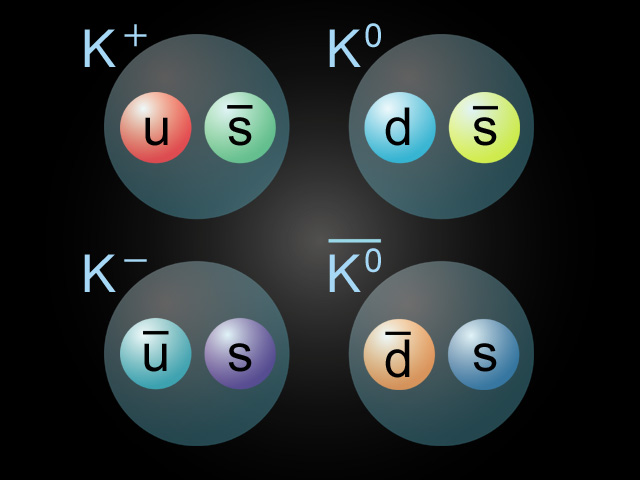
\includegraphics[height=0.6\textheight]{Images/Kaonen.png}
            \caption{Übersicht über die Kaonen}
          \end{center}
        \end{figure}
      \end{column}
      \begin{column}{0.5\textwidth}
        Kaonen:
        \begin{itemize}
          \item sind die leichtesten Teilchen mit Strangeness $S = \pm1$
          \item besitzen einen ganzzahligen Spin
          \item sind Bosonen
          \item verfügen über eine relativ lange Lebensdauer
        \end{itemize}
        \begin{table}
          \centering
          \begin{tabular}{
              S[table-format=6.0]
              S[table-format=3.5]
              @{${}\pm{}$}
              S[table-format=1.5]
              S[table-format=3.4]
              @{${}\pm{}$}
              S[table-format=1.4]
            }
              \toprule
              & \multicolumn{2}{c}{$m \:/\: \si{\mega\electronvolt}$} & \multicolumn{2}{c}{$\tau \:/\: 10^{-10} \si{\second}$} \\
              \midrule
              $K^{\pm}$   & 493.677 & 0.016 & 123.80 & 0.21 \\
              $K⁰_{S}$    & 497.614 & 0.024 & 0.8954 & 0.0004 \\
              $K⁰_{L}$    & 497.614 & 0.024 & 511.6  & 2.1 \\
              ${\pi}^{\pm}$ & 139.57018 & 0.00035 & 260.33 & 0.05 \\
              \bottomrule
          \end{tabular}
        \end{table}
      \end{column}
    \end{columns}
  \end{frame}

\section{Historische Kaonenexperimente}
  \begin{frame}{Weltkarte}
    %Hier könnte ihre Weltkarte stehen
  \end{frame}

\subsection{Entdeckung der Kaonen}
  \begin{frame}{Entdeckung der Kaonen}
    \begin{columns}[onlytextwidth]
      \begin{column}{0.4\textwidth}
        \begin{figure}[ht]
          \begin{center}
            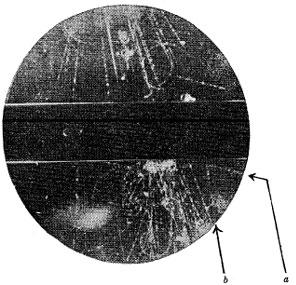
\includegraphics[height=0.6\textheight]{Images/Kaondiscovery.png}
            \caption{Nebelkammeraufnahme der kosmischen Höhenstrahlung von Rochester und Butler 1947}
          \end{center}
        \end{figure}
      \end{column}
      \begin{column}{0.5\textwidth}
        \begin{itemize}
          \item Entdeckung des ersten (neutralen) Kaons 1947 durch George Rochester et. al
          \item Höhenstrahlung wurde in Nebelkammer untersucht
          \item Zerfall eines neutralen Teilchens in ein positives und negatives Pion
          \begin{equation*}
            K^{0} \rightarrow \pi^{+} \pi^{-}
          \end{equation*}
          \item Entdeckung des positiv geladenen Kaons 1949 durch Powell in Kernreaktionen
          \item Zerfall eines positiven Kaons in zwei positive und ein negatives Pion
          \begin{equation*}
            K^{+} \rightarrow \pi^{+} \pi^{+} \pi^{-}
          \end{equation*}
        \end{itemize}
      \end{column}
    \end{columns}
  \end{frame}

  \begin{frame}{Seltsam lange Lebensdauer}
    \begin{columns}[onlytextwidth]
      \begin{column}{0.4\textwidth}
        \begin{figure}[ht]
          \begin{center}
            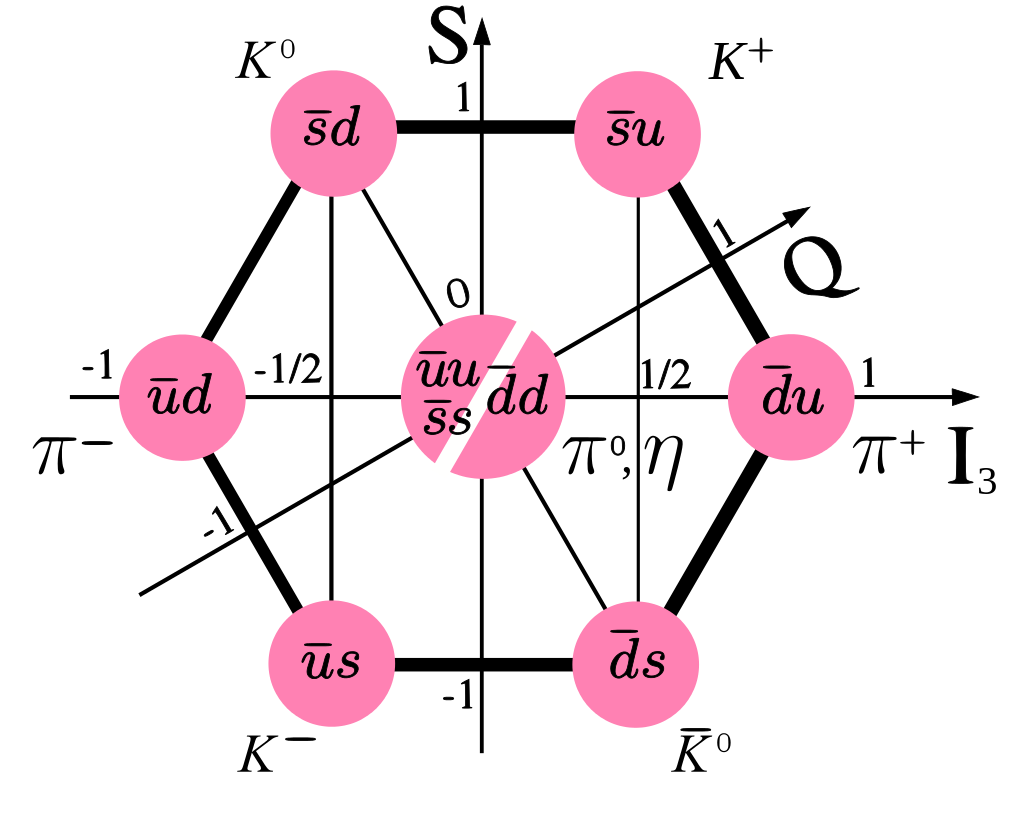
\includegraphics[height=0.6\textheight]{Images/Meson-octet.png} %Zuschnippeln
            \caption{Der achtfache Weg von Gell-Mann und Ne'eman}
          \end{center}
        \end{figure}
      \end{column}
      \begin{column}{0.5\textwidth}
        \begin{itemize}
          \item Sehr leichte Erzeugung (durch starke WW)
          \item Sehr langsamer Zerfall $10^{-10}\si{\second}$ (durch schwache WW)
          \item Gell-Mann 1953: Einführung einer neuen Teilcheneigenschaft/ Quantenzahl \item[\rightarrow] Strangeness
          \item Zerfall sehr leicht möglich, wenn \textbf{S} durch alle Kräfte erhalten wäre
          \item[Aber:] Zerfall nur über die flavourändernde schwache WW möglich
          %\item \textbf{S} veranlasste Cabibo 1963 zur Postulierung des Cabibo-Winkels
        \end{itemize}
      \end{column}
    \end{columns}
  \end{frame}

\subsection{Paritätsverletzung}

  \begin{frame}{Paritätsverletzung und der Cosmotron}
    \begin{columns}[onlytextwidth]
      \begin{column}{0.4\textwidth}
        \begin{figure}[ht]
          \begin{center}
            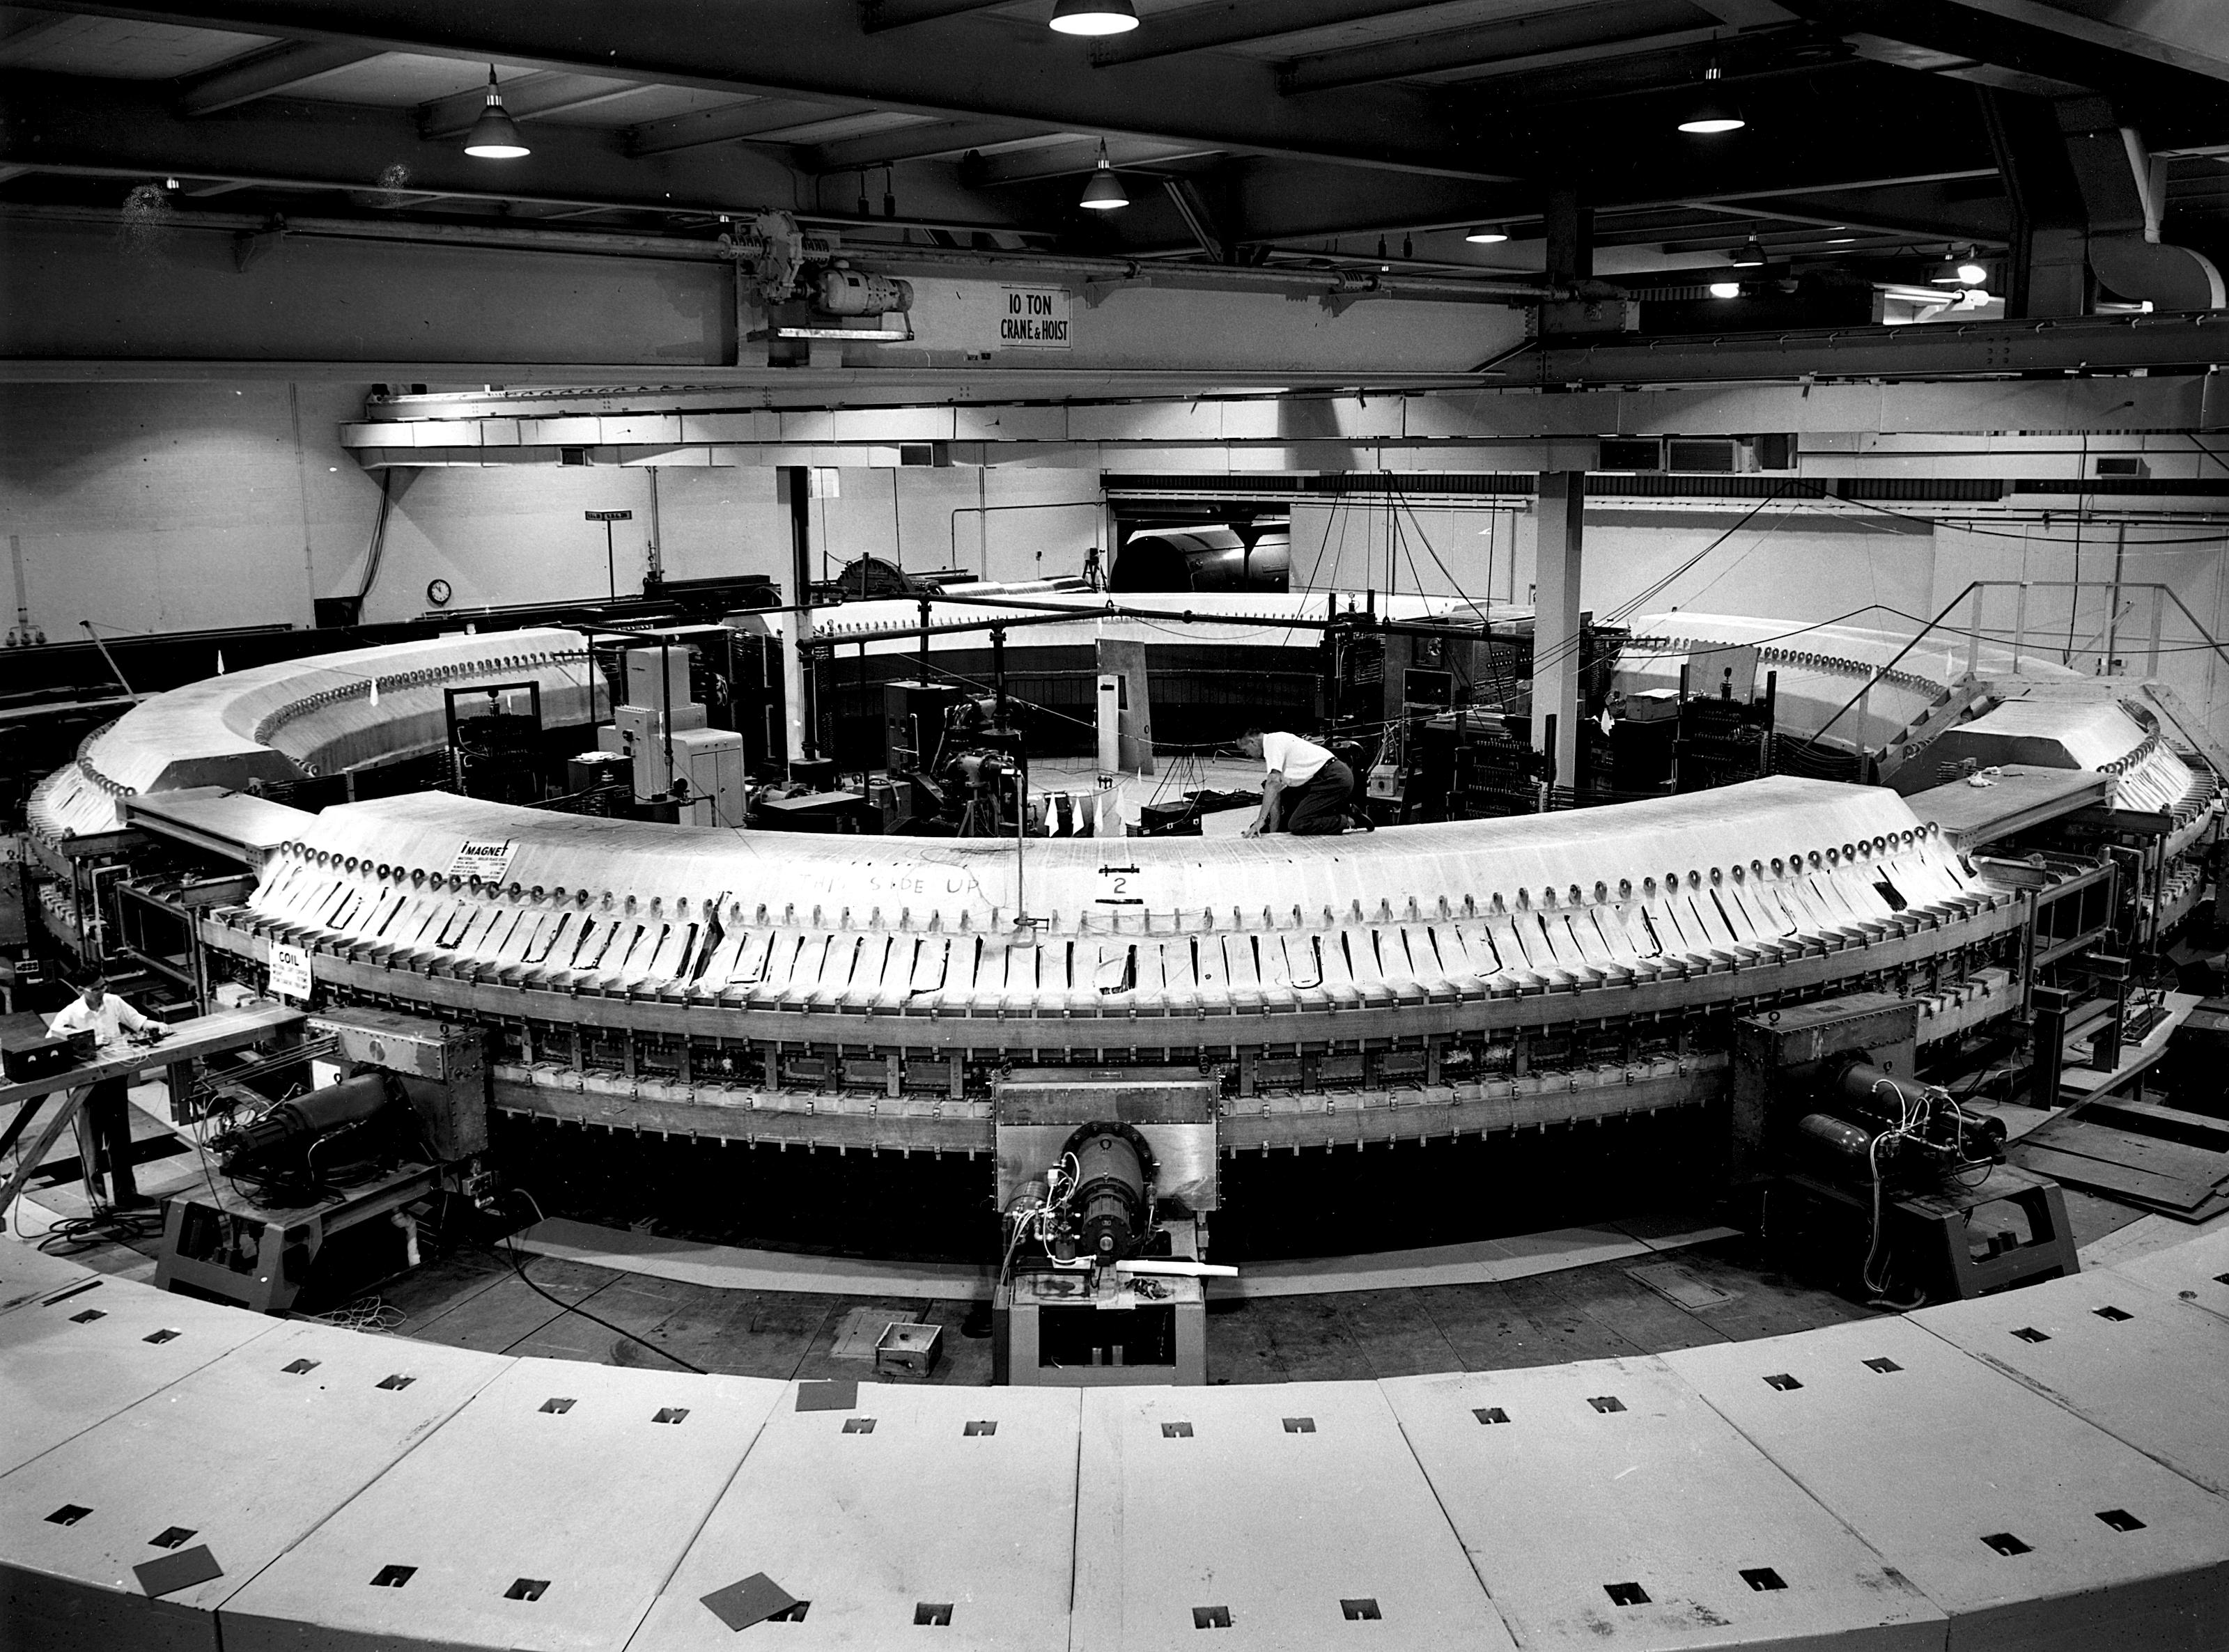
\includegraphics[height=0.6\textheight]{Images/cosmotron.jpg} %Zuschnippeln
            \caption{Das Cosmotron am Brookhaven National Laboratory (1952-1966)}
          \end{center}
        \end{figure}
      \end{column}
      \begin{column}{0.5\textwidth}
        \begin{itemize}
          \item Leistungsstärkstes Proton-Synchrotron (1952) mit Strahlenergien von $\SI{3.3}{\giga\electronvolt}$
          \item Erstmals Produktion von schweren Teilchen der kosmischen Höhenstrahlung
          \item Entdeckung $K_{L}$ durch Lande (1956) %in Nebelkammer
          \item Beobachtung der Zerfälle
          \begin{align*}
            \tau^{+} \rightarrow \pi^{+} \pi^{+} \pi^{-} \\
            \theta^{+} \rightarrow \pi^{+} \pi^{0}
          \end{align*}
          \item[] durch T.D. Lee und C.N.Yang (1956)
          \item $\tau^{+}$ und $\theta^{+}$ tatsächlich $K^{+}$
          \item[\rightarrow] Zerfälle verletzen die Paritätserhaltung
        \end{itemize}
      \end{column}
    \end{columns}
  \end{frame}

\subsection{Kaonenmischung}

  \begin{frame}{Long und short? Die Mischung neutraler Kaonen}
    \begin{columns}[onlytextwidth]
      \begin{column}{0.4\textwidth}
        \begin{figure}[ht]
          \feynmandiagram[layered layout, horizontal=a to b, scale=0.9]{
            i1 [particle=\(d\)]
              -- [fermion] a
              -- [photon, edge label=\(W^{-}\)] b
              -- [fermion] f1 [particle=\(\overline s\)],
            i2 [particle=\(\overline s\)]
              -- [anti fermion] c
              -- [photon, edge label'=\(W^{-}\)] d
              -- [anti fermion] f2 [particle=\(d\)],
            { [same layer] a -- [fermion, edge label'=\(u\, c\, t\)] c },
            { [same layer] b -- [anti fermion, edge label=\(u\, c\, t\)] d}
          };
        \end{figure}
        \begin{figure}[ht]
          \feynmandiagram[layered layout, horizontal=a to b, scale=0.9]{
            i1 [particle=\(d\)]
              -- [fermion] a
              -- [fermion, edge label=\(u\, c\, t\)] b
              -- [fermion] f1 [particle=\(\overline s\)],
            i2 [particle=\(\overline s\)]
              -- [anti fermion] c
              -- [anti fermion, edge label'=\(u\, c\, t\)] d
              -- [anti fermion] f2 [particle=\(d\)],
            { [same layer] a -- [photon, edge label'=\(W^{-}\)] c },
            { [same layer] b -- [photon, edge label=\(W^{-}\)] d}
          };
        \end{figure}
      \end{column}
      \begin{column}{0.5\textwidth}
        \begin{itemize}
          \item Flavour-Eigenzustände $\ket{K^{0}}$, $\ket{\overline{K^{0}}}$ unterscheiden sich von den CP-Eigenzuständen:
          \begin{equation*}
            \begin{drcases*}
              CP \ket{K^{0}} = \ket{\overline{K^{0}}} \\
              CP \ket{\overline{K^{0}}} = \ket{K^{0}}
            \end{drcases*}
            \rightarrow
            \begin{cases}
              \ket{K_1} = \frac{1}{\sqrt{2}}\left(\ket{K^{0}} + \ket{\overline{K^{0}}} \right) \\
              \ket{K_2} = \frac{1}{\sqrt{2}}\left(\ket{K^{0}} - \ket{\overline{K^{0}}} \right)
            \end{cases}
          \end{equation*}
          \item Dabei ist $\ket{K_1} \approx \ket{K_{S}}$ und $\ket{K_2} \approx \ket{K_{L}}$
          \begin{equation*}
            \tau(\ket{K_{L}}) \approx 600 \times \tau(\ket{K_{S}})
          \end{equation*}
          \item $\ket{K_{S}}$ haben CP = +1 und $\ket{K_{L}}$ habe CP =-1
          \item Unterschied vor allem in Zerfallsmoden:
          \begin{align*}
            \ket{K_{S}} &\rightarrow \pi^{+} \pi^{-} \\ %Mehr Möglichkeiten im Phasenraum
            \ket{K_{L}} &\rightarrow \pi^{+} \pi^{-} \pi^{0} %Eigentlich verboten, s.h. später
          \end{align*}
        \end{itemize}
      \end{column}
    \end{columns}
  \end{frame}

\subsection{Direkte und indirekte CP-Verletzung}

  \begin{frame}{CP-Verletzung}
    \begin{columns}[onlytextwidth]
      \begin{column}{0.4\textwidth}
        \begin{figure}[ht]
          \begin{center}
            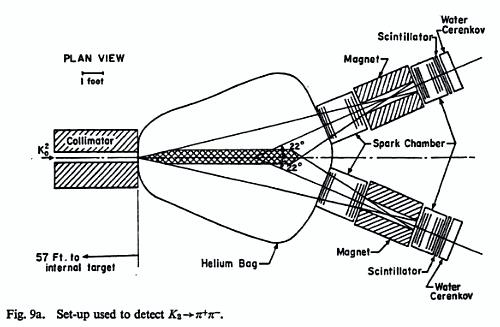
\includegraphics[height=0.6\textheight]{Images/croninfitch.png} %Zuschnippeln
            \caption{Das Cronin-Fitch-Experiment am Brookhaven National Laboratory (1964)}
          \end{center}
        \end{figure}
      \end{column}
      \begin{column}{0.5\textwidth}
        \begin{itemize}
          \item Planung 1964 durch Christenson, Cronin, Fitch und Turlay am Brookhaven National Laboratory %Collimator => Bündelung de Teilchenstrahlen
          \item $\SI{17}{\metre}$ lange Beamline
          \item[\rightarrow] Zerfall der $\ket{K_{S}}$
          \item Messung des Winkels $\theta$ zwischen $K_{L}^{0}$-Strahl und Teilchenimpulsen
          \item Bestimmung der Winkelsumme bei 'gleichzeitiger' Detektion
          \item Für Dreikörperzerfall mit großer Wahrscheinlichkeit $\neq 0$
          \item Für Zweikörperzerfälle hingegen mit großer Wahrscheinlichkeit $= 0$
        \end{itemize}
      \end{column}
    \end{columns}
  \end{frame}

  \begin{frame}{Ergebnis}
    \begin{columns}[onlytextwidth]
      \begin{column}{0.4\textwidth}
        \begin{figure}[ht]
          \begin{center}
            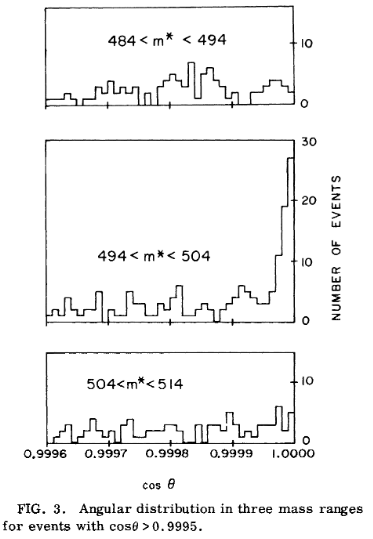
\includegraphics[height=0.8\textheight]{Images/croninfitch_erg.png}
            \caption{Ergebnis der Winkelmessung}
          \end{center}
        \end{figure}
      \end{column}
      \begin{column}{0.5\textwidth}
        \newline
        \newline
        \newline
        \newline
        Tatsächlich wurd der Zerfall
        \begin{align*}
          K_{L} \rightarrow \pi^{+} \pi^{-}
        \end{align*}
        gemessen.
      \end{column}
    \end{columns}
  \end{frame}

  \begin{frame}{Wie kann das sein?}
    \begin{itemize}
      \item Konsequenz: $\ket{K_{S}}$ und $\Ket{K_{L}}$ keine reinen CP- Zustände
      \item[\rightarrow] Indirekte CP-Verletzung
      \item[\rightarrow] Beide Zustände enthalten kleine Teile des anderen Zustands:
      \begin{align*}
        \ket{K_{L}^0} &= \frac{\epsilon \ket{K_1} + \ket{K_2}}{\sqrt{1 + \epsilon^2}} \\
        \ket{K_{S}^0} &= \frac{\ket{K_1} + \epsilon \ket{K_2}}{\sqrt{1 + \epsilon^2}} \\
        |\epsilon| &= (2.229\pm0.010)\times10^{-3}
      \end{align*}
      \item Neutrale Kaonenzustände oszillieren über Box-Diagramme und zerfallen
      \item Oder direkte CP-Verletzung über Pinguin- Diagramme
      \item Problem: Im Jahre 1964 noch keine Quarks oder der CKM-Mechanismus bekannt
    \end{itemize}
  \end{frame}

  \begin{frame}{Direkte CP- Verletzung}
    \begin{columns}[onlytextwidth]
      \begin{column}{0.4\textwidth}
        \begin{figure}[ht]
          \begin{tikzpicture}
            \begin{feynman}
              \vertex(a1){\(\overline s\)};
              \vertex[right=2cm of a1] (a2);
              \vertex[right=0.5cm of a2] (a3);
              \vertex[right=0.5cm of a3] (a4);
              \vertex[right=2cm of a4] (a5){\(\overline d\)};

              \vertex[below=2cm of a1] (b1){\(d\)};
              \vertex[below=2cm of a5] (b2){\(d\)};

              \vertex[below=1.5em of a5] (c1){\(u\)};
              \vertex[above=1.5em of b2] (c3){\(\overline u\)};
              \vertex at ($(c1)!0.5!(c3)- (1cm, 0)$) (c2);

              \diagram* {
                {[edges=fermion]
                  (a5)-- (a4)-- (a3)-- (a2)-- (a1),
                },
                (b1)-- [fermion] (b2),
                (c3)-- [fermion,out=180,in=-60] (c2)-- [fermion,out=60,in=180] (c1),
                (a3)-- [gluon, bend right, edge label'=\(g\, Z\, \gamma\)] (c2),
                (a4)-- [boson,out=90,in=90,looseness=2.0,edge label'=\(W\)] (a2)
              };

              \draw[decoration={brace}, decorate] (b1.south west)-- (a1.north west)
                node[pos=0.5, left] {  \(K^{0}\)};
              \draw[decoration={brace}, decorate] (a5.north east)-- (c1.south east)
                node[pos=0.5, right] {  \(\pi^{+}\)};
              \draw[decoration={brace}, decorate] (c3.north east)-- (b2.south east)
                node[pos=0.5, right] {  \(\pi^{-}\)};
            \end{feynman}
          \end{tikzpicture}
          \caption{Pinguindiagramm des CP-verletzenden, neutralen Kaonenzerfalls}
        \end{figure}
      \end{column}
      \begin{column}{0.5\textwidth}
        \begin{itemize}
          \item Direkte CP-Verletzung:
          \item[\rightarrow] Keine vorherige Mischung der Kaonen
          \item Messung der partiellen Zerfallsbreiten von:
          \begin{align*}
            K_{L}^0 &\rightarrow \pi^+ \pi^- \\
            K_{L}^0 &\rightarrow \pi^0 \pi^0 \\
            K_{S}^0 &\rightarrow \pi^+ \pi^- \\
            K_{S}^0 &\rightarrow \pi^0 \pi^0
          \end{align*}
          \item Bildung der Verhältnisse
          \item[\rightarrow] Anteile der direkten und indirekten Verletzung spielen eine Rolle
        \end{itemize}
      \end{column}
    \end{columns}
  \end{frame}

  \begin{frame}{Was wird dann gemessen?}
    \begin{columns}[onlytextwidth]
      \begin{column}{0.4\textwidth}
        \begin{align*}
          \eta_{00} = \frac{A \left(K_L \rightarrow \pi^0 \pi^0 \right)}{A \left(K_S \rightarrow \pi^0 \pi^0 \right)} &= \epsilon - 2 \epsilon^{\prime} \\
          \eta_{\pm} = \frac{A \left(K_L \rightarrow \pi^+ \pi^- \right)}{A \left(K_S \rightarrow \pi^+ \pi^- \right)} &= \epsilon +  \epsilon^{\prime}
        \end{align*}
        \begin{equation*}
          %R = \frac{A \left(K_L \rightarrow \pi^0 \pi^0 \right)}{A \left(K_S \rightarrow \pi^0 \pi^0 \right)} / \frac{A \left(K_L \rightarrow \pi^+ \pi^- \right)}{A \left(K_S \rightarrow \pi^+ \pi^- \right)}
          \symup{Re}(\epsilon' / \epsilon) = \frac{1}{6} \left\{1 - \left|\frac{\eta_{00}}{\eta_{\pm}}\right|^2 \right\}
        \end{equation*}
        %\begin{equation*}
        %  \approx 1 - 6 \,\symup{Re}(\epsilon^{\prime} / \epsilon)
        %\end{equation*}
      \end{column}
      \begin{column}{0.5\textwidth}
        \begin{itemize}
          \item Vorteil: Viele systematische Fehler kürzen sich
          \item $\epsilon^{\prime} = 0$: keine direkte CP-Verletzung
          \item $\epsilon^{\prime} \neq 0$: direkte CP-Verletzung
          \item Bis in die 90er kein eindeutiges Ergebnis durch Experimente
        \end{itemize}
        Theoretische Überlegungen:
        \begin{itemize}
          \item Drei Quarkfamilien (Kobayashi und Maskawa, 1973) % \rightarrow noch vor Entdeckung des Charm-Quarks)
        \end{itemize}
        Experimentelle Implikationen:
        \begin{itemize}
          \item Drei Generationen messbar
          \item Beobachtung direkter CP-Verletzung in Mesonen-Systemen
        \end{itemize}
      \end{column}
    \end{columns}
  \end{frame}

  \section{Moderne Experimente}

  \subsection{Motivation für moderne Kaon-Experimente}

  \begin{frame}{Motivation}
    Warum sind Kaonen-Experimente immer noch wichtig für das Verständnis fundamentaler Fragen der Teilchenphysik?
    \begin{itemize}
      \item Gibt es noch weitere Ursachen für CP-Verletzung, abseits der komplexen Phase der CKM-Matrix?
      \item Inwieweit ist die Leptonuniversalität berücksichtigt?
      \item Wie weit können die Grenzen der Hochenergie-Teilchenphysik in Bezug auf seltene Prozesse gebracht werden?
      \item Gibt es neue Physik, die man durch die Untersuchung von mesonischen Loopzerfällen, beobachten kann?
      \item Können fundamentale Symmetrien, wie CPT, untersucht werden und wenn ja bis zu welchem Grad?
    \end{itemize}
  \end{frame}

  \subsection{Zurück zu direkter CP-Verletzung}

  \begin{frame}{Wer war an der Messung von Re$(\epsilon^{\prime} / \epsilon)$ beteiligt?}
    KTeV am FermiLab
    \begin{itemize}
      \item Vorläufer: E731 \rightarrow Re$(\epsilon^{\prime} / \epsilon) = (7.4\pm5.9) \times10^{-4}$
      \item Kaons at the TeVatron
    \end{itemize}
    NA48 am Cern
    \begin{itemize}
      \item Vorläufer NA31 \rightarrow Re$(\epsilon^{\prime} / \epsilon) = (23.0\pm6.5) \times10^{-4}$
      \item North Area 48
      %\item Fixed target mit $\SI{450}{\giga\electronvolt}$ vom SPS
      %\item Gleichzeitige Messung von $\ket{K_L}$ und $\ket{K_S}$ durch Strange-Tagging
    \end{itemize}
  \end{frame}

  \subsection{NA48}

  \begin{frame}{Das Experiment NA48}
    \begin{figure}
      
\includegraphics[height=0.8\textheight]{Images/ripcern.png}
    \end{figure}
  \end{frame}

  \begin{frame}
    \begin{columns}[onlytextwidth]
      \begin{column}{0.4\textwidth}
        \begin{figure}[ht]
          \begin{center}
            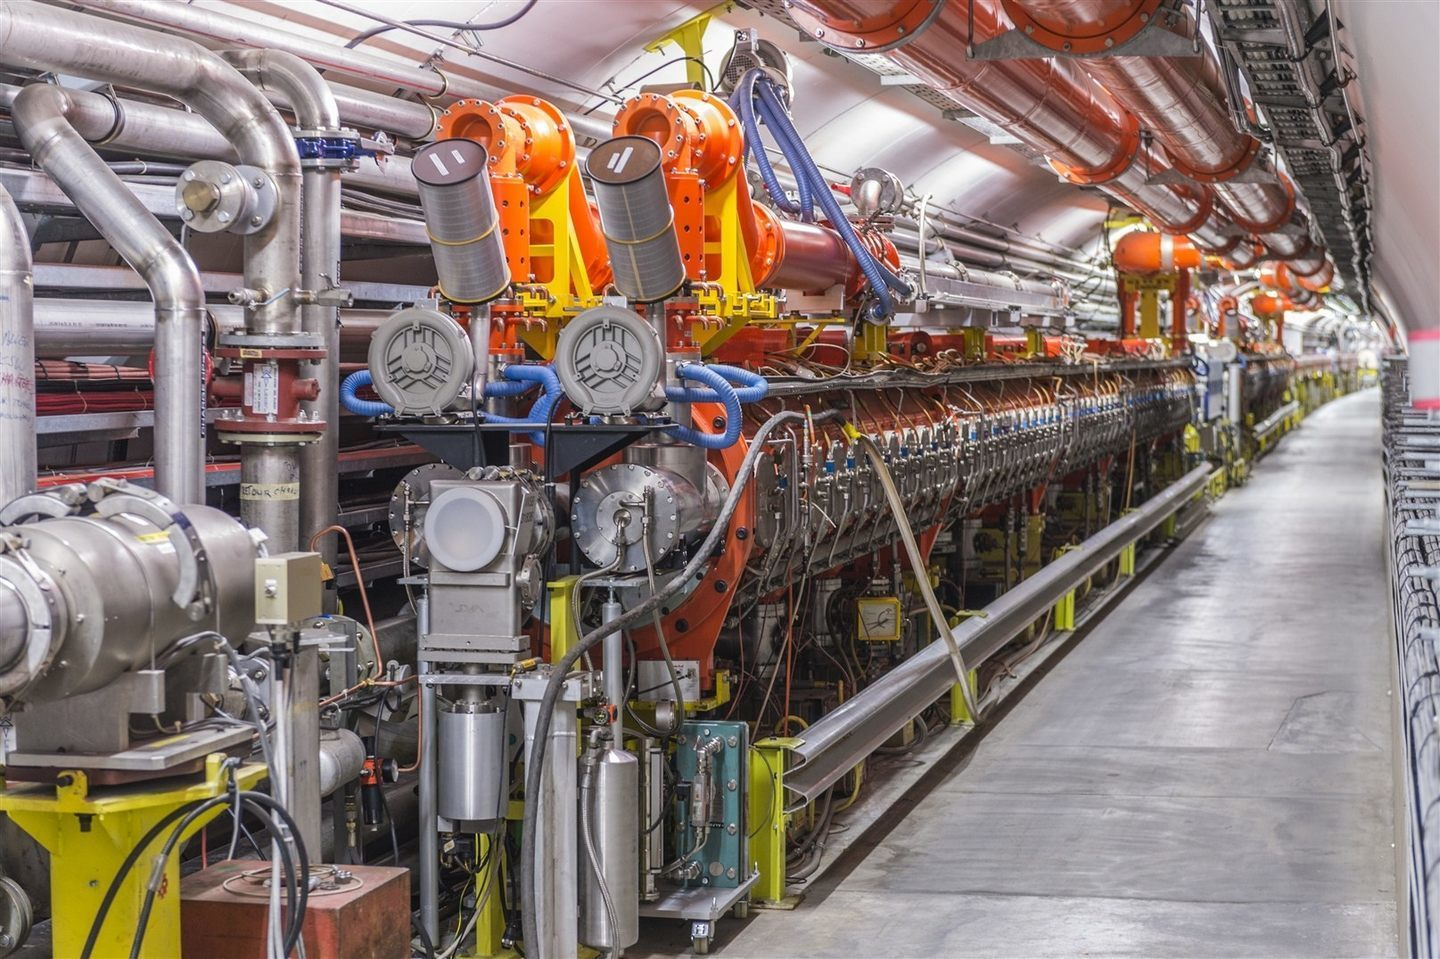
\includegraphics[width=\textwidth]{Images/sps.jpg} %Zuschnippeln
            \caption{Tunnel des Super Proton Synchrotrons (SPS)}
          \end{center}
        \end{figure}
      \end{column}
      \begin{column}{0.5\textwidth}
        \begin{itemize}
          \item Fixed target mit $\SI{450}{\giga\electronvolt}$ vom SPS
          \item Gleichzeitige Messung von $\ket{K_L}$ und $\ket{K_S}$ durch $K_S$-Tagging
          \item Trennung von $\ket{K_L}$ und $\ket{K_S}$ nach letztem Collimator
          \item Auftreffen von $\ket{K_L}$ und $\ket{K_S}$ am gleichen Detektorpunkt
          \item Vertexrekonstruktion ausreichend für Zerfall in geladene $\pi$
          \item Tagging ermöglicht zeitliche Trennung
        \end{itemize}
      \end{column}
    \end{columns}
  \end{frame}

  \begin{frame}{Aufbau der NA48 Beamline}
    \begin{figure}[ht]
      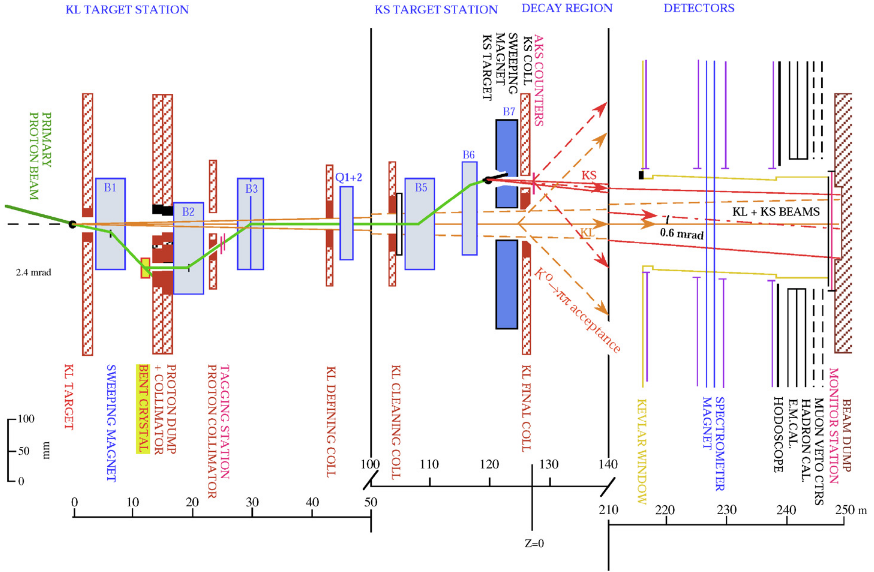
\includegraphics[height=0.95\textheight]{Images/na48quer.png}
      \caption{Beamline des NA48-Experiments}
    \end{figure}
  \end{frame}

  \begin{frame}{$K_S$-Tagging}
    \begin{columns}[onlytextwidth]
      \begin{column}{0.4\textwidth}
        \begin{figure}[ht]
          \vspace*{-1cm}
          \begin{center}
            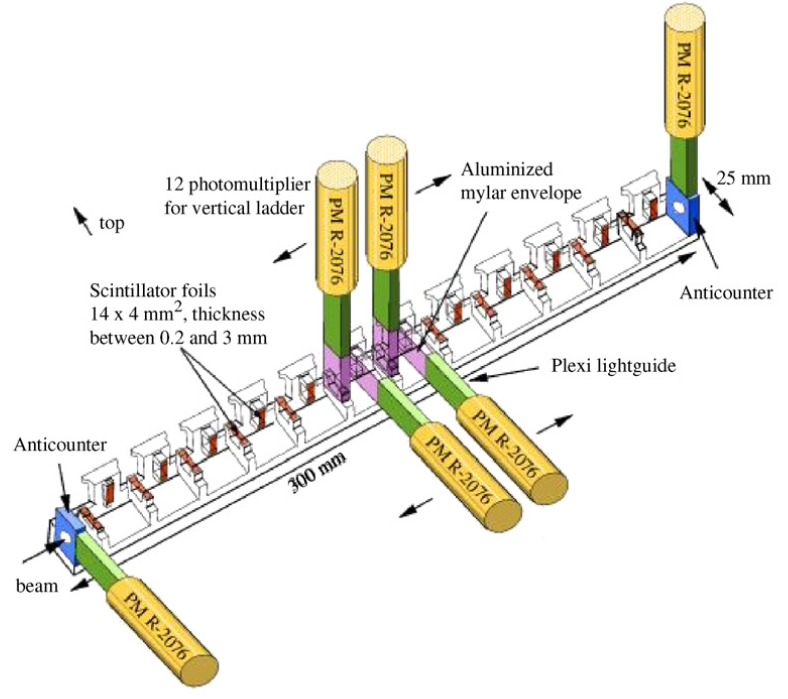
\includegraphics[height=0.8\textheight]{Images/na48strangetag.png} %Zuschnippeln
            \caption{Schema des NA48-Taggings}
          \end{center}
        \end{figure}
      \end{column}
      \begin{column}{0.5\textwidth}
        \begin{itemize}
          \item Zerfall in $\pi^0$ problematisch
          \item Zuordnung durch Messung der Zeitdifferenz
          \item Tagging eines Protons vor $K_S$-Target
          \item Überprüfen der Zeit der Detektion durch LKr-Calorimeter
          \item[\rightarrow] Zuordnung möglich
        \end{itemize}
      \end{column}
    \end{columns}
  \end{frame}

\subsection{Aufbau des NA48-Detektors}

  \begin{frame}{Detektor}
    \begin{figure}[ht]
      \begin{center}
        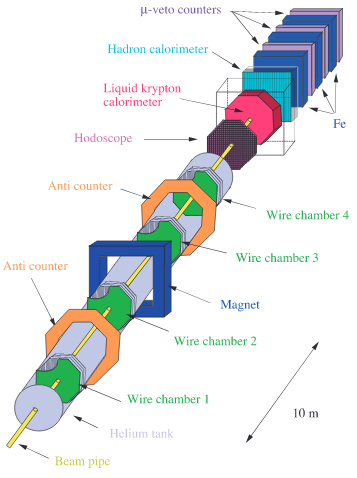
\includegraphics[height=0.8\textheight]{Images/na48detector.png} %Zuschnippeln
        \caption{Detektor des NA48-Experiments}
      \end{center}
    \end{figure}
  \end{frame}

  \begin{frame}{Heliumtank}
    \begin{itemize}
      \item Geschützt durch hochstabiles Kevlar-Glas
      \item Atmosphärendruck
      \item Beherbergt Spektrometer und Wire chambers %Driftkammern
      \item[\rightarrow] Genutzt zur Bestmmung der Winkel von geladenen $\pi$
      \item[\rightarrow] Beherbergt dafür Eisenjochmagnet ($\SI{0.37}{\tesla}$ im Zentrum)
    \end{itemize}
  \end{frame}

  \begin{frame}
    \begin{figure}[ht]
      \begin{center}
        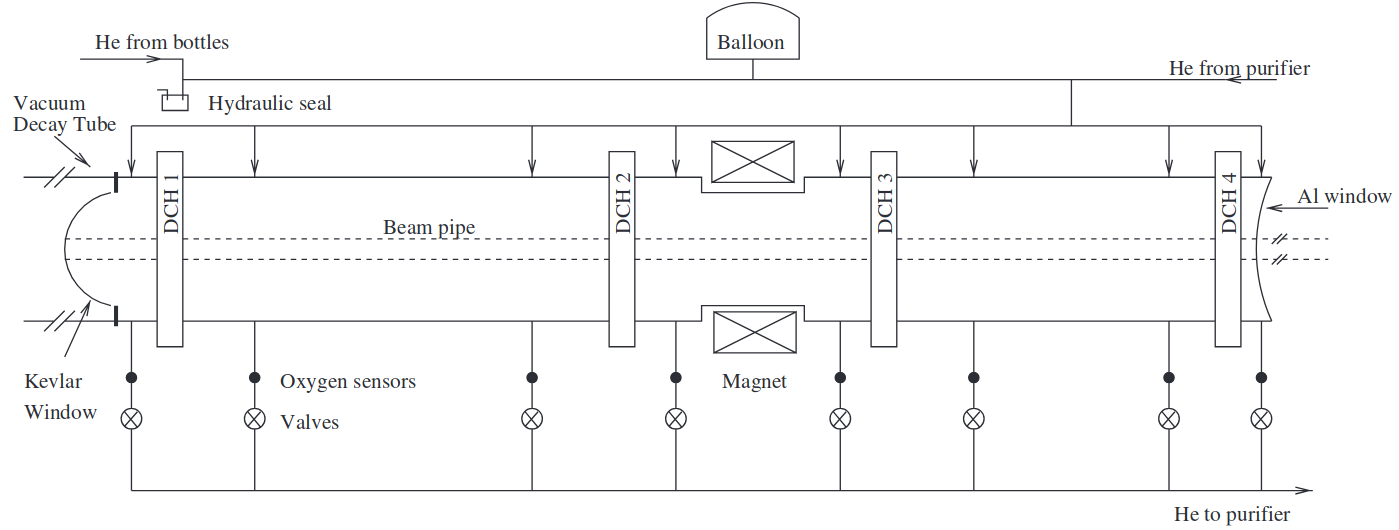
\includegraphics[width=0.9\textwidth]{Images/na48helium.png} %Zuschnippeln
        \caption{Schema des Heliumtanks aus NA48 mit Spektrometern}
      \end{center}
    \end{figure}
  \end{frame}

  \begin{frame}{Hodoskop}
    \begin{columns}[onlytextwidth]
      \begin{column}{0.4\textwidth}
        \begin{figure}[ht]
          \begin{center}
            \vspace*{-1cm}
            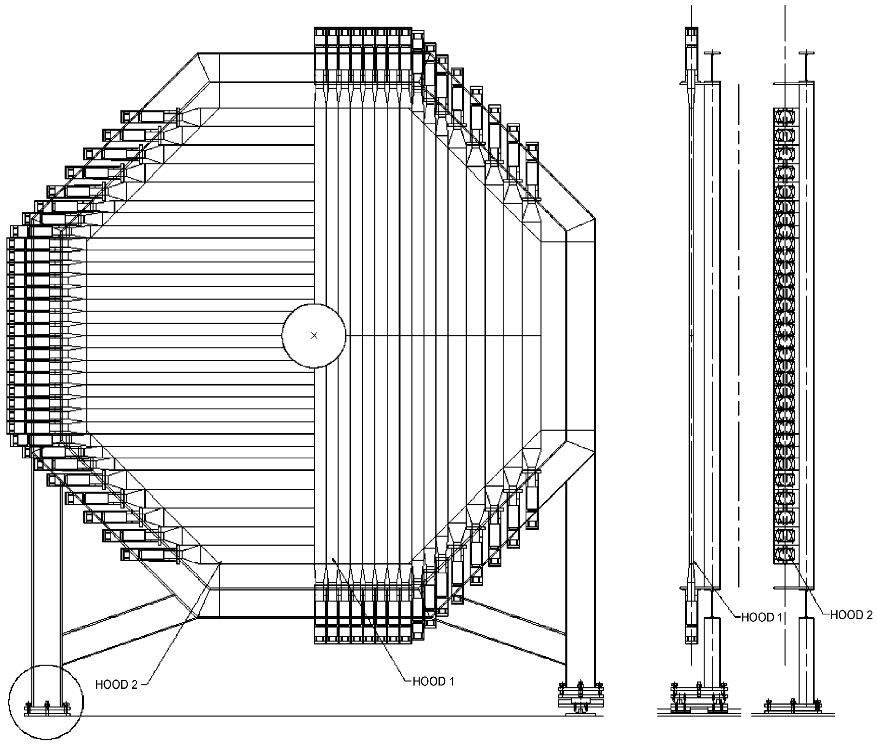
\includegraphics[height=0.8\textheight]{Images/na48chodoskop.png} %Zuschnippeln
            \caption{Detektor des NA48-Experiments}
          \end{center}
        \end{figure}
      \end{column}
      \begin{column}{0.5\textwidth}
        \begin{itemize}
          \item Griechisch für Pfadseher
          \item System aus Plastik-Szintillatoren und Photomultipliern
          \item[\rightarrow] 64x64 Szintillatoren im Abstand von $\SI{74}{\centi\metre}$
          \item Signal für Zerfall in geladene $\pi$
        \end{itemize}
      \end{column}
    \end{columns}
  \end{frame}

  \begin{frame}{Flüssig-Krypton-Kalorimeter}
    \begin{columns}[onlytextwidth]
      \begin{column}{0.4\textwidth}
        \begin{figure}[ht]
          \begin{center}
            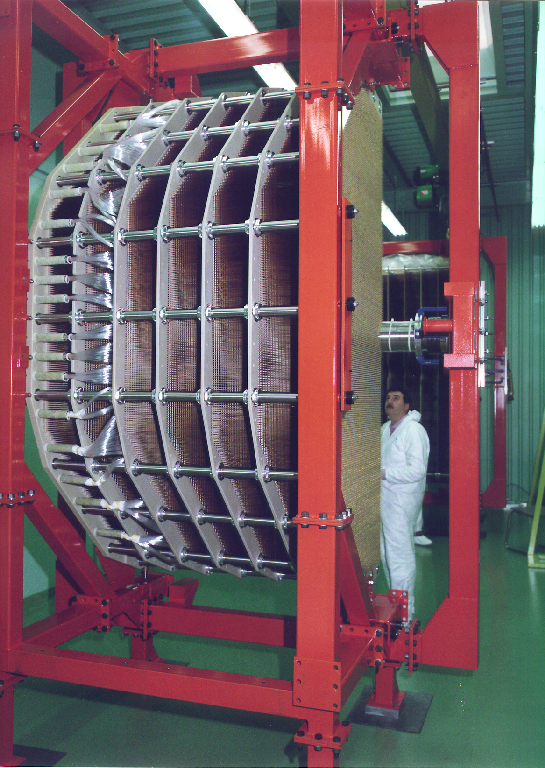
\includegraphics[height=0.7\textheight]{Images/na48lkr.png} %Zuschnippeln
            \caption{Das LKr-Kalorimeter vor dem Einbau}
          \end{center}
        \end{figure}
      \end{column}
      \begin{column}{0.5\textwidth}
        \begin{itemize}
          \item Hohe Granularität und Energieauflösung
          \item Hauptsächlich zur Detektion von:
          \begin{equation*}
            \pi^0 \rightarrow \gamma \gamma
          \end{equation*}
          \item Bestimmung der $\gamma$-Energie und Transversalimpulse
          \item Funktion ähnlich einer normalen Ionisationskammer
          \item[\rightarrow] Stabiles Signal bei hoher Reinheit
          \item[\rightarrow] Korreliert gut mit der Energie der eingehenden $\gamma$ und $e^-$
          \item Echtzeitmessung zum taggen der $\pi^0$
          \item Unterdrückung des Untergrunds durch semileptonische Zerfälle %zufällig gleiche Masse
        \end{itemize}
      \end{column}
    \end{columns}
  \end{frame}

  \begin{frame}{Hadronen-Kalorimeter} %nicht sehr spannend
    \begin{columns}[onlytextwidth]
      \begin{column}{0.4\textwidth}
        \begin{figure}[ht]
          \begin{center}
            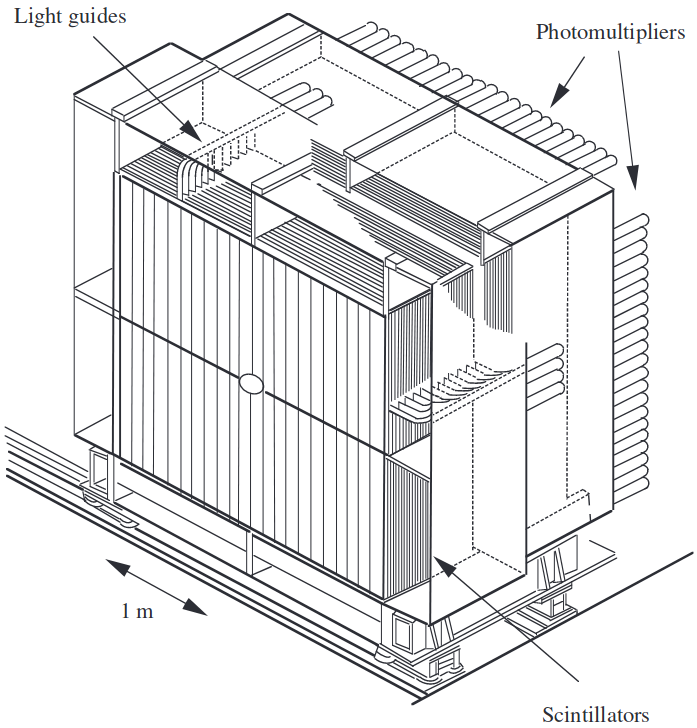
\includegraphics[height=0.7\textheight]{Images/na48hac.png} %Zuschnippeln
            \caption{Schema des hadronischen Kalorimeters von NA48}
          \end{center}
        \end{figure}
      \end{column}
      \begin{column}{0.5\textwidth}
        \begin{itemize}
          \item Messung der Energie und Position der Teilchenschauer innerhalb des Detektors
          \item Hauptsächlich zum Triggern genutzt
          \item[\rightarrow] Trigger auf Gesamtenergie und als Veto für neutrale Teilchen
          \item[\rightarrow] $\pi^0$ sollten vor EM-Kalorimeter in $2\gamma$ zerfallen
          \item[Rest:] Andere Zerfälle (Hintergrund)
        \end{itemize}
      \end{column}
    \end{columns}
  \end{frame}

  \begin{frame}{Die $\mu$-Veto-Counter}
    \begin{itemize}
      \item $\mu$-Kammern zur Detektion von
      \begin{equation*}
        K_S \rightarrow \mu \mu \mu
      \end{equation*}
      \item[] Zerfällen
      \item Ausgestattet mit Szintillations-Hodoskopen zur Bahnberechnung
      \item Abgeschirmt durch dicke Eisenwände
      \item[\rightarrow] Anordnung analog zu neueren Experimenten, z.B. LHCb und ATLAS
    \end{itemize}
  \end{frame}

  \begin{frame}{$K_S$ Anti-Counter}
    \begin{columns}[onlytextwidth]
      \begin{column}{0.4\textwidth}
        \begin{figure}[ht]
          \begin{center}
            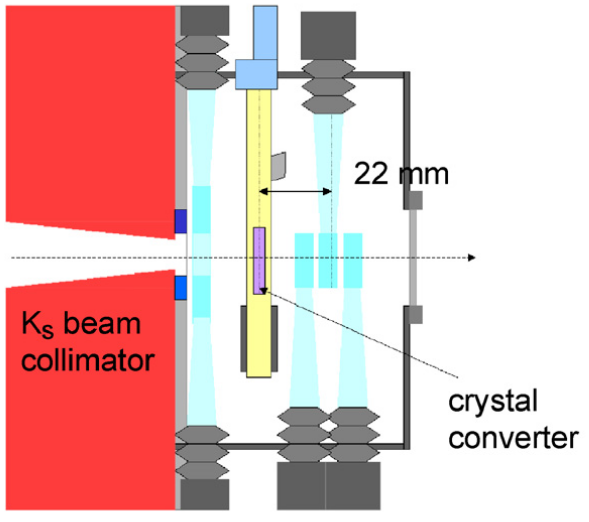
\includegraphics[height=0.7\textheight]{Images/na48aks.png} %Zuschnippeln
            \caption{Aufbau des $K_S$ Anti-Counters}
          \end{center}
        \end{figure}
      \end{column}
      \begin{column}{0.5\textwidth}
        \begin{itemize}
          \item Veto-Trigger von Zerfällen außerhalb der Wire-Chambers und Kalorimetern
          \item[\rightarrow] Veto von Zerfällen in geladen Teilchen
        \end{itemize}
      \end{column}
    \end{columns}
  \end{frame}

  \begin{frame}{$K_S$ Anti-Counter}
    \begin{columns}[onlytextwidth]
      \begin{column}{0.4\textwidth}
        \begin{figure}[ht]
          \begin{center}
            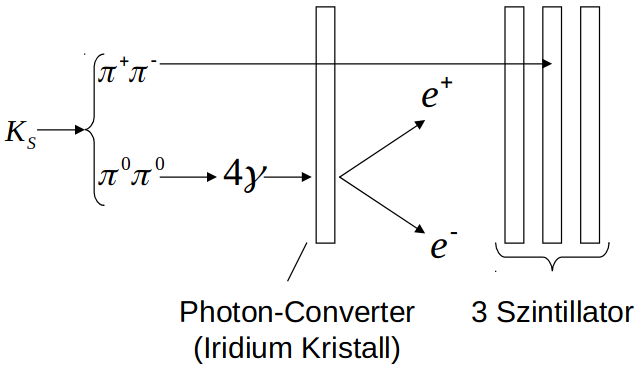
\includegraphics[width=1.2\textwidth]{Images/na48aksschema.png} %Zuschnippeln
            \caption{Schema des $K_S$ Anti-Counters}
          \end{center}
        \end{figure}
      \end{column}
      \begin{column}{0.5\textwidth}
        \begin{itemize}
          \item Veto-Trigger von Zerfällen außerhalb der Wire-Chambers und Kalorimetern
          \item[\rightarrow] Veto von Zerfällen in geladen Teilchen
        \end{itemize}
      \end{column}
    \end{columns}
  \end{frame}

  \subsection{KTeV}

  \begin{frame}{Das KTeV-Experiment}
    \begin{figure}
      
\includegraphics[height=0.8\textheight]{Images/rip.png}
    \end{figure}
  \end{frame}

  \begin{frame}
    \begin{columns}[onlytextwidth]
      \begin{column}{0.4\textwidth}
        \begin{figure}[ht]
          \begin{center}
            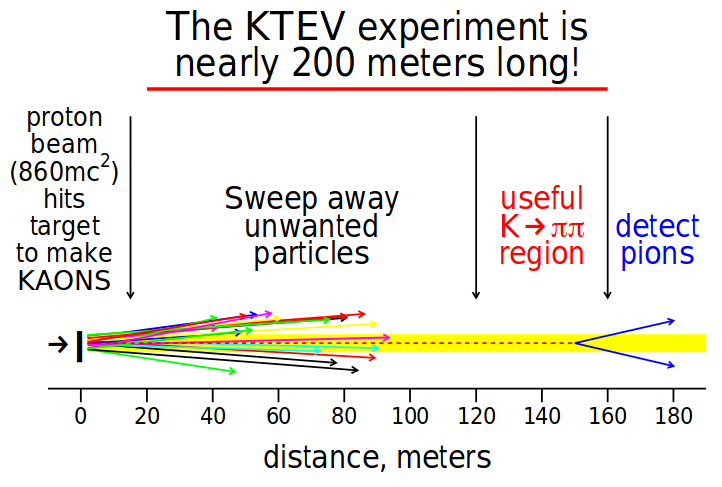
\includegraphics[height=0.6\textheight]{Images/ktevdistance.png} %Zuschnippeln
            \caption{Konzept des KTeV Experiments}
          \end{center}
        \end{figure}
      \end{column}
      \begin{column}{0.5\textwidth}
        \begin{itemize}
          \item Kaonzerfall im Vakuum um Kollision mit Luft zu verhindern
          \begin{align*}
            K^0 &\rightarrow \pi^+ \pi^- \\
                &\rightarrow \pi^0 \pi^0
          \end{align*}
          \item $\pi$-Impulse werden durch die Krümmung ihrer Bahnen gemessen (Magnetfeld)
          \item Anschließend Spurmessung durch 'wire chambers'
          \item $\pi$ die Detektor verfehlen, werden simuliert und berücksichtigt
        \end{itemize}
      \end{column}
    \end{columns}
  \end{frame}

  \begin{frame}
    \begin{figure}[ht]
      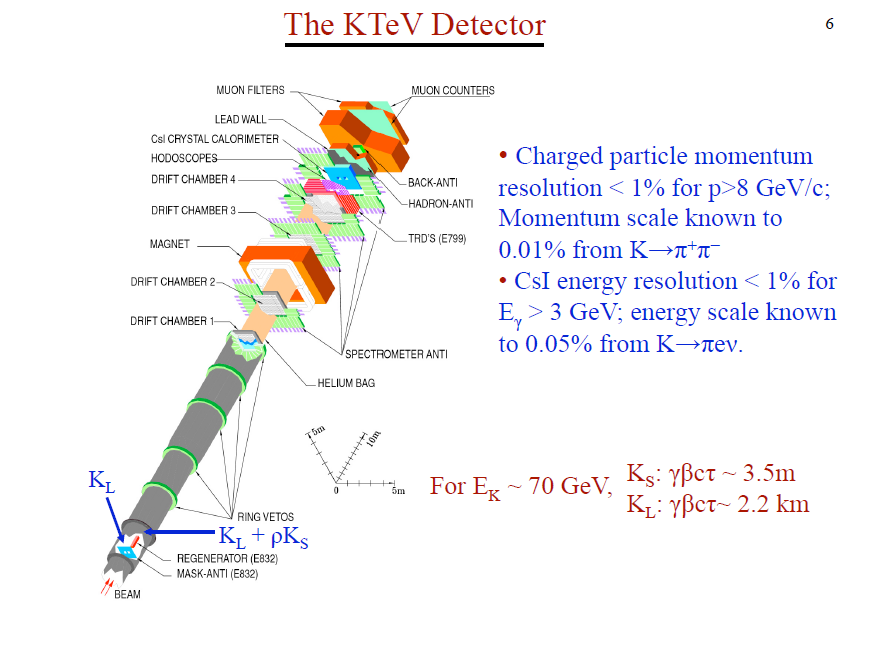
\includegraphics[height=0.8\textheight]{Images/KTEVDETEKTOR.png}
      \caption{Detektor des KTeV-Experiments}
    \end{figure}
  \end{frame}

  \subsection{Ergebnisse von KTeV und NA48}

  \begin{frame}{Ergebnisse beider Experimente}
    \begin{figure}
      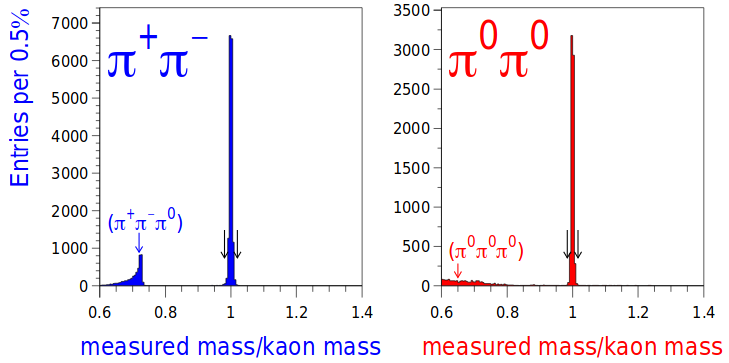
\includegraphics[height=0.8\textheight]{Images/ktevdata.png}
      \caption{Massenverteilung von KTeV}
    \end{figure}
  \end{frame}

  \begin{frame}
    \begin{figure}
      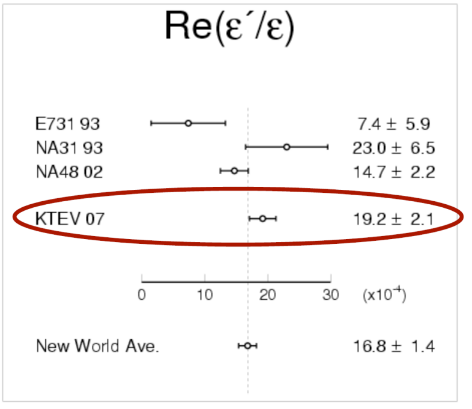
\includegraphics[height=0.7\textheight]{Images/ktevaverage.png}
    \end{figure}
    KTeV Ergebnis: Re$(\epsilon' / \epsilon) = (19.2\pm2.1) \times 10^{-4}$ (Stand: 2009)
    \newline
    Weltdurchschnitt: Re$(\epsilon' / \epsilon) = (16.8\pm1.4) \times 10^{-4}$
  \end{frame}

  \begin{frame}
    \begin{figure}[ht]
      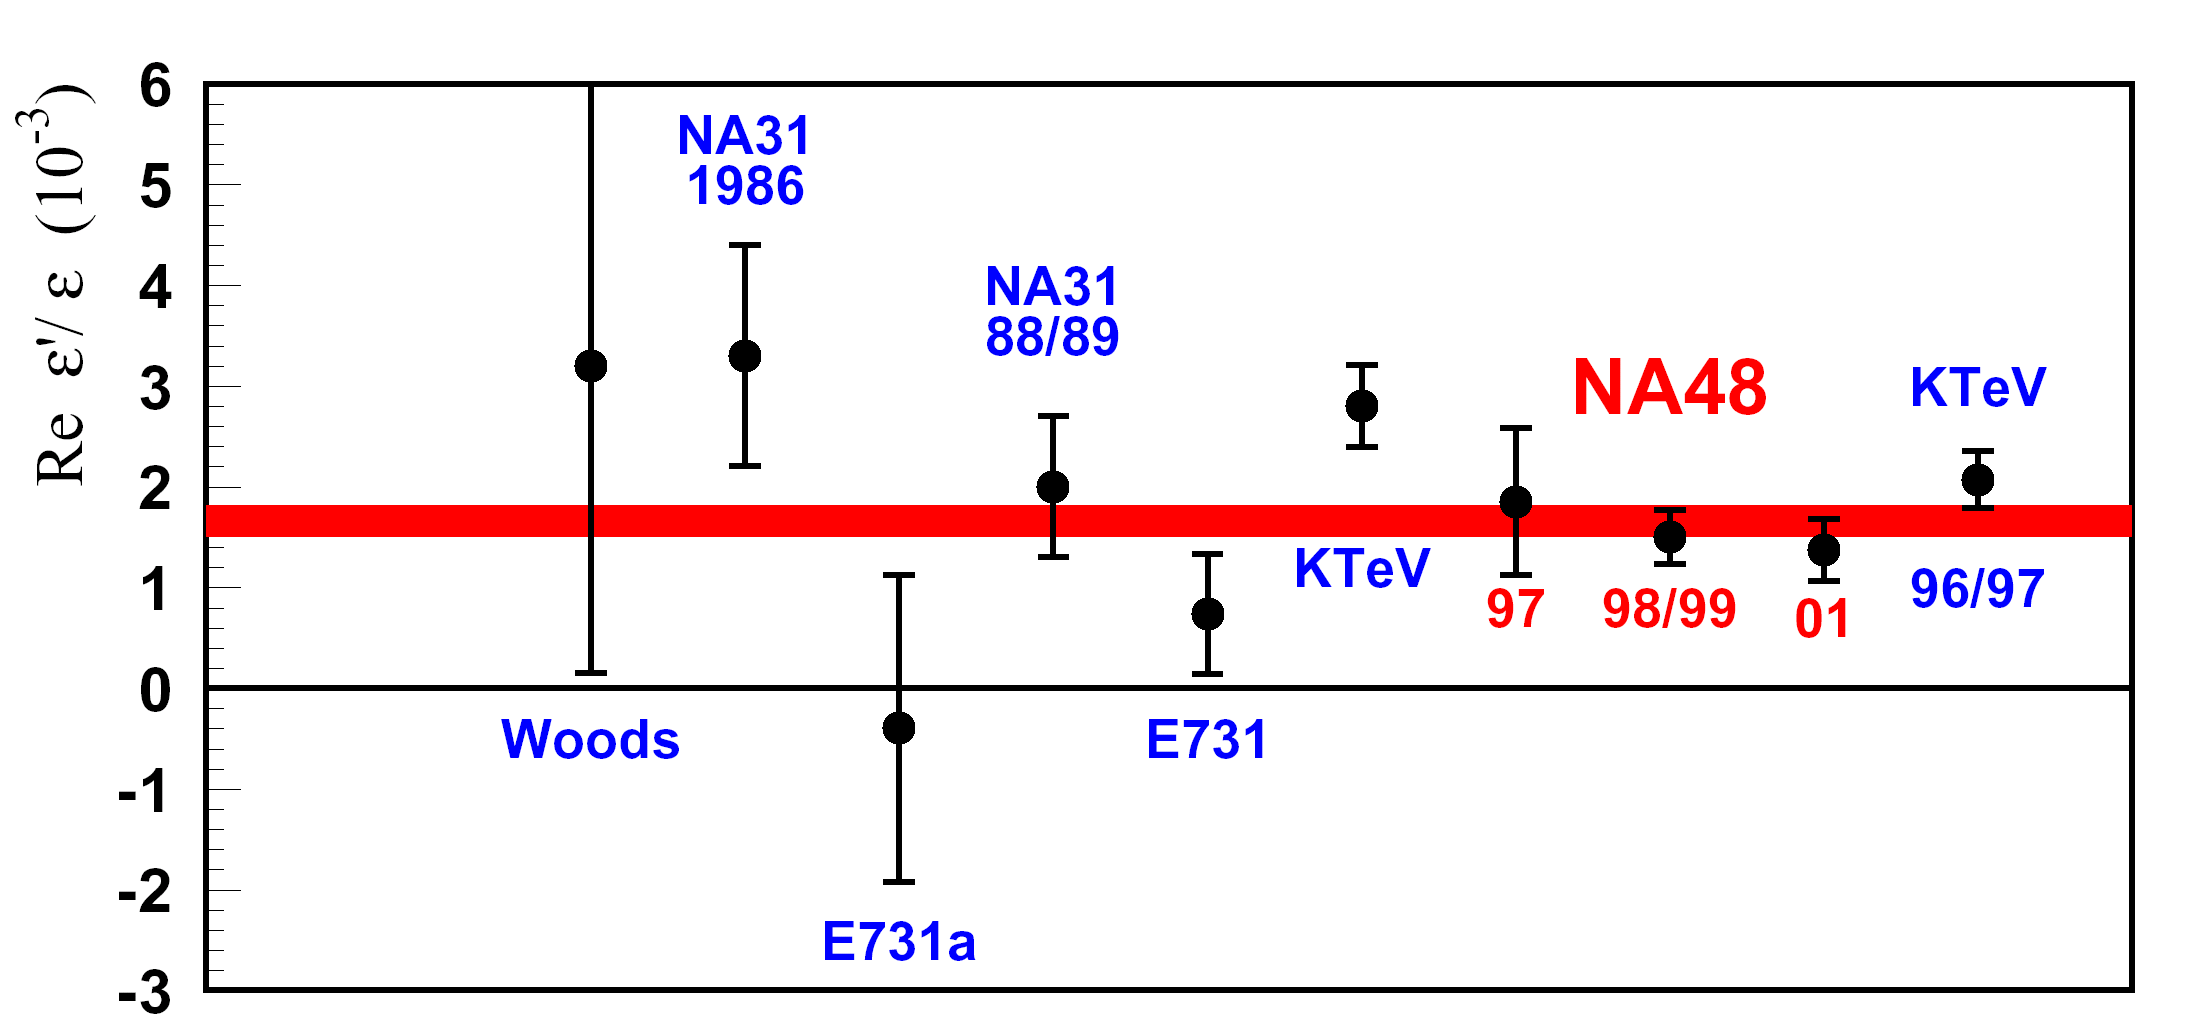
\includegraphics[height=0.8\textheight]{Images/REEE.png}
      \caption{Ergebnisse für Re$(\epsilon' / \epsilon) $}
    \end{figure}
  \end{frame}

\section{Seltene Zerfälle}

  \subsection{Aussehen und Motivation}

  \begin{frame}{Aussehen und Motivation}
    \begin{figure}[ht]
      \feynmandiagram[vertical=e to f] {
      a -- [fermion, edge label=\(s\)] b -- [photon, edge label=\(W\)] c -- [fermion, edge label=\(d\)] d,
      b -- [fermion, edge label'=\(t\)] e -- [fermion, edge label'=\(t\)] c,
      e -- [boson, edge label=\(Z\)] f,
      h -- [fermion, edge label=\(\bar{\nu}\)] f -- [fermion, edge label=\(\nu\)] i;
      };
      \caption{Pinguindiagramm des CP-verletzenden, neutralen Kaonenzerfalls}
    \end{figure}
  \end{frame}



%\section{Kaptel 2}
  %\begin{frame}{Folie 2.1}
    %Text
  %\end{frame}

\end{document}
